\textbf{$\ket{\phi^-}=\frac{1}{\sqrt{2}} (\ket{00}-\ket{11})$} \vspace{.3cm}

\begin{quote}
    \begin{minted}[fontsize=\small, linenos, frame=single]{python}
estado_inicial = [0,1]
circuito_bell2 = QuantumCircuit(2)
circuito_bell2.initialize(estado_inicial,0)
circuito_bell2.h(0)
circuito_bell2.cx(0,1)                #cx: controlled x
circuito_bell2.measure_all()
circuito_bell2.draw('mpl')
    \end{minted}
    \vspace{.3cm}
    \begin{center}
        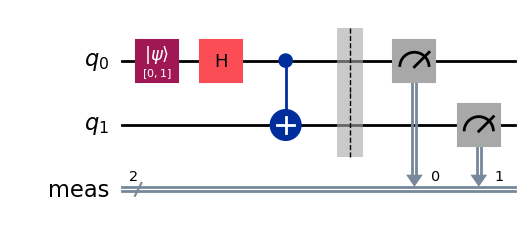
\includegraphics[height=3.3cm]{src/Img/3.1.png}
    \end{center}

    Para crear todos los estados de Bell en realidad se utiliza casi el mismo circuito con
    diferentes estados iniciales, es decir con diferentes qubits iniciales. En este caso pasa:

    \begin{align*}
        \hat{C_x}\hat{H}\ket{10}
        = \hat{C_x} \left( \frac{1}{\sqrt{2}} (\ket{00}-\ket{10}) \right)
        = \frac{1}{\sqrt{2}} (\ket{00}-\ket{11})
    \end{align*}

    Podemos comprobar sacando el statevector, recordando que la base es $00,01,10,00$.
    \vspace{.5cm}

    \begin{center}
        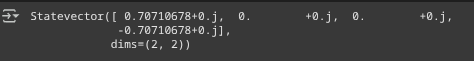
\includegraphics[width=.8\textwidth]{src/Img/3.1.r.png}
    \end{center}
\end{quote}
\vspace{.5cm}
